% Todo:

\documentclass[12pt]{article}
\usepackage{xeCJK}
\usepackage{fontspec}
%\setCJKmainfont{SimSun}
\setCJKmainfont[BoldFont=SimHei,ItalicFont=KaiTi]{SimSun}
\setCJKsansfont{SimHei}
\setCJKmonofont{KaiTi}
\setmainfont{Arial}

\usepackage{cite}
\usepackage{graphicx}
\usepackage{float}
\usepackage{amsfonts}
% \usepackage{amsmath}	% for \tag
\usepackage{amssymb}	% for \multimap
% \usepackage{stmaryrd}
\usepackage{color}
%\usepackage[square,numbers]{natbib}
%\nocopyright
%\usepackage{latexsym,amsmath,amssymb,graphicx,hyperref}
%\usepackage{times} % gives you a bit more space if needed
\usepackage{titlesec}		% change color of section headings
\usepackage{verbatim} % for block comments

\titleformat{\section}
{\color{blue}\normalfont\Large\bfseries}
{\color{blue}\thesection}{1em}{}
\renewcommand\abstractname{\textcolor{blue}{Abstract}}

\newcommand{\concept}[1]{\textbf{\textcolor{blue}{#1}}}
% \definecolor{LogicColor}{rgb}{0.4,0.1,0.4}  % Magenta
\definecolor{grey}{rgb}{0.4,0.4,0.4}
\definecolor{LogicColor}{rgb}{0.4,0.1,0.4}  % Magenta

\newcommand{\english}[1]{\rmfamily \textit{``#1''}\rmfamily}
\newcommand{\formula}[1]{\textcolor{LogicColor}{#1}}
% \newcommand{\formula}[1]{\ttfamily\textcolor{LogicColor}{#1}\rmfamily}

\newcommand{\df}{f} %probability density function
\newcommand{\dfo}{f1} %other probability density function
\newcommand{\fv}{x} %fuzzy variable
\newcommand{\tab}{\hspace*{1cm}}
\newcommand{\zand}{\; \tilde{\wedge} \;}
\newcommand{\zor}{\; \tilde{\vee} \;}
\newcommand{\PimpL}{\leftarrowtriangle}
\newcommand{\com}{\multimap}
\newcommand{\comL}{\circ \hspace{-0.4em} - \,}
\newcommand{\mul}{}
\newcommand{\loves}{loves }
\newcommand{\heart}{\, \heartsuit \,}

\setlength{\oddsidemargin}{1cm}
\setlength{\evensidemargin}{1cm}
\setlength{\textwidth}{14cm}

\title{\textcolor{blue}{Genifer 3.0 白皮书}}
\author{YKY (\textit{甄景贤})}
% \institute{}

\begin{document}

\tab\tab\tab \parbox{11cm}{\textit{我是个发烧友,但不是疯子,因为我对於如何建构飞机有些心得。 我希望分享我所知的一切,然后,如可能的话,出一分力去帮助那将来会达到最终成功的人。}}
\vspace{-0.5cm}
\begin{flushright}
\textemdash \, Wilbur Wright
\end{flushright}

% \sffamily

{\let\newpage\relax\maketitle}

\maketitle
\setlength{\parindent}{0em}
\setlength{\parskip}{1.5ex plus0.5ex minus1.2ex}

\begin{abstract}
\noindent 介绍通用人工智能\  Genifer 3 的理论。\\
写得很仓促,如看不懂请提问。
\end{abstract}

\section{背景}

Genifer 3 是「新古典主义」的、基於逻辑的人工智能,和 OpenCog、NARS 等相似。 在 Genifer 4 我企图脱离经典逻辑,转移到向量空间中使用连续逼近法,但其具体细节现在仍未落实。 

\concept{命题逻辑}关心的是有\textbf{真假值}的命题,原子命题没有\textbf{内部结构}。 例如,可以有这个逻辑式子: $P \wedge Q$。  命题逻辑是 isomorphic to Boolean algebra。  在命题逻辑中做逻辑推导,是著名的 NP-complete 问题,叫「可判定性」(\concept{satisfiability}, SAT)。  \concept{Resolution} (消解原理)是命题逻辑的推导算法。

\concept{谓词逻辑}赋予命题的内部结构,例如: \formula{爱(小明, 小娟)}。  谓词逻辑容许有一些 patterns 例如 \formula{爱(X, Y)} ,其中 X,Y 是\textbf{变量}。  这些模式要和实际句子做配对 (pattern-matching),这配对的算法叫归一化 (\concept{unification})。  例如,以下这式子定义「爷爷」的概念:\\
\tab\formula{爷爷(X, Z) $\leftarrow$ 爸爸(X, Y) $\wedge$ 爸爸(Y, Z)}。

谓词逻辑的推导算法,需要结合 unification 和 resolution。  结合后,算法的复杂性在最差情况下是可以\textbf{没有终止}的 (non-terminating): 因为一阶逻辑是 Turing universal,而「停机定理」(halting problem) 证明了这样的逻辑推导不存在必然会回覆的算法。

Genifer 3 与经典逻辑有以下区别:
\begin{itemize}
\item 用 fuzzy-probabilistic (机率/模糊) 的真假值
\item 不使用变量 (variables)
\end{itemize}

Fuzzy-probabilistic 推导法的原理很简单,属例行公事,但因为要服从机率的法则,需要用到 \concept{Bayesian belief propagation} (机率传播算法)。

不使用变量的原因是因为变量的思维方式很\textbf{不自然}。 例如人类认识「爷爷」这概念,是「爸爸的爸爸」(在关系代数中记作 \formula{爸爸 $\circ$ 爸爸}),而不是像 \formula{X 是 Y 的爸爸} 这样使用变量。 而且,在推导过程中,变量令我们需要做颇复杂的 substitution management,这在经典的 \textit{``Structure and Interpretation of Computer Programs''} 中有详细描述,但我们可以不理。 例如,图中所示,谓词逻辑的式子中,变量之间的连结 (binding) 关系可以很复杂: 
\begin{figure}[H]
\centering
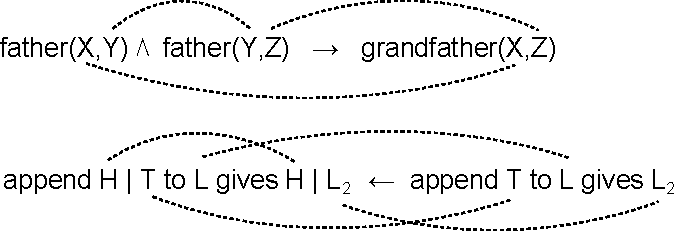
\includegraphics[scale=0.8]{connections-logic-variables.pdf}
\caption{\textcolor{grey}{谓词逻辑中变量之间的连结: 「爷爷」的定义,和 PROLOG 中将一个序列 append 到另一个序列的定义。}}
\end{figure}

\concept{组合逻辑} (combinatory logic) 是一种没有变量的逻辑;  而 \concept{关系代数} (relation algebra) 也是一种组合逻辑,但局限在关系的运算上。 Genifer 3 使用的是一种简化的关系代数。

AI 的瓶颈在於其\concept{学习算法},在下文会讨论。

\section{逻辑}

Genifer 3 的逻辑式子很简单,就是一串原子\concept{概念} (atomic concepts) 的乘积:\\
\tab $c_1 \cdot c_2 \cdot ... \cdot c_n$.\\
例如:  \formula{小明 $\cdot$ 爱 $\cdot$ 小娟}.

由於不使用变量,Genifer 3 需要利用\concept{包含}关系 $\subseteq$,例如:\\
\tab \formula{猫 $\subseteq$ 动物}。\\
这关系容许逻辑上的\concept{一般化} (generalization) ,例如,从「人是会死的」推导到「苏格拉底会死」。

一个逻辑式子,可以是\concept{事实} (fact) 或\concept{规则} (rule);  规则的特点是具有前件、后件的结构:\\
\tab \formula{pre-condition $\rightarrow$ post-condition}。

作为例子,考虑如何从这些已知事实:\\
\tab \formula{小明 $\cdot$ 爸爸 = 小强} \tab (小明的爸爸是小强)\\
\tab \formula{小强 $\cdot$ 爸爸 = 大强}\\
推导出这个新的事实:\\
\tab \formula{小明 $\cdot$ 爷爷 = 大强}。

这个问题可以用规则 \formula{爸爸 $\cdot$ 爸爸 = 爷爷},再用代入 (substitution) 的方式解决,但我暂时还不肯定可不可将这动作化简为更\textbf{原始}的操作?

\section{动作 (actions)}

不使用变量的逻辑可能会变得太弱,意思是失去 Turing universal。  补救的办法是使用「记忆储存器」。 

大家记得 Turing machine 包含一条读写磁带和有限个状态的转移规则:
\begin{figure}[H]
\centering
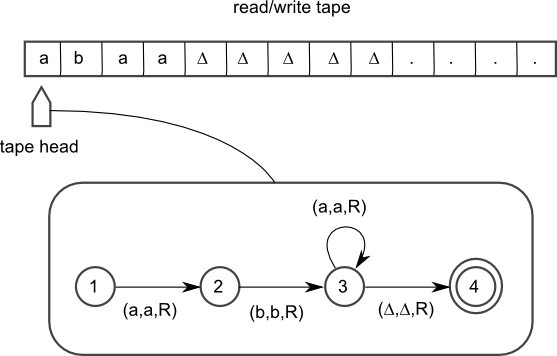
\includegraphics[scale=0.75]{Turing-machine.png}
\caption{\textcolor{grey}{接受 aba* 的图灵机。}}
\end{figure}

如果我们在逻辑上加上某种记忆体,就自然地可以重获 Turing universal。 

具体地说:\\
\tab \formula{下雨了 $\rightarrow$ 草地是湿的}\\
是一句经典逻辑句子,但我们可以引入一种带有\textbf{动作}的逻辑句子:\\
\tab \formula{如果储存器 A 的值是 0 $\rightarrow$ 将 1 写入储存器 B}。\\
甚至我们不使用个别的储存器,而是用一些资料结构,例如 linked list 或 tree。 在 Genifer 3.0 我尝试用 list。

\begin{comment}
我们有了动作 但不知道怎样指向\textbf{对象}。 其中一个可能的办法是 用 label 标签上次的答案;  或者作用於所有答案(但这是不自然的?) 

这引申到注意力的问题。  或者 Genifer 永远只是 focus 在注意力的前沿?

还有个问题就是:答案并不一定是唯一的。 所以需要一个方法去把 KB 的答案 掟回到 register 里。  

但那又引申到 working memory 和 KB 的区别。  或者 attention 只是 derivation 的 time-decaying trace?  换句话说,那些可能的答案只有很少几个。  我们应该可以利用某些特徵提取他们。

最简单可能就是 -1 和「没有」的分别。  如何区别「有」和「没有」呢?  可以指定答案的 class,例如「广东话字词」。
\end{comment}

\section{学习}

学习的目的是寻找一组逻辑式子去\textbf{解释}这世界。  所谓解释即推导。

学习的方法是 inductive learning,即由事实\concept{诱导}出法则 (induce rules from facts)。

用逻辑表达就是:\\
\tab $KB \cup H \models E$\\
其中 KB 是\concept{知识库} (knowledge base) 或\textbf{背景知识},H 是我们想学习的新的\concept{假设} (hypothesis),E 是一些实例 (examples),或者可以说是新的经验 (experiences),学习的目的是用 H + KB 去解释这些新经验,$\models$ 表示逻辑\concept{蕴涵} (entailment)。

Inductive learning 就是\textbf{在所有可能的逻辑句子空间中搜寻},这个空间异常地大。 这空间如果有\concept{格} (lattice) 的序结构,搜寻会快很多。  那就是 \concept{general-to-specific order}。  传统逻辑中这个\concept{序}可以由两种方法达成:
\begin{enumerate}
\item 某个概念比另一个概念更\textbf{一般},例如:\\
\tab \formula{ 动物 $\supseteq$ 狗 }
\item conjunctions 的增加,例如:\\
\tab \formula{ 戴眼镜 $\wedge$ 长头发 } 比 \formula{长头发} 更\textbf{特殊}。
\end{enumerate}

在 Genifer 4 我企图用连续空间的梯度下降法,但这条路线离成功还很远。  Genifer 3 不需要连续空间,那就只需用 genetic algorithm 去学习,这样很容易。 容易未必表示不好,例如在机器学习比赛的实践中,人们发现最有效率的分类算法是理论上很简单的决策树 (decision tree),而不是理论很复杂的支持向量机 (SVM)。 可能 Genifer 3 用进化/遗传算法已经足够?

\begin{comment}
压缩的方法必须是 ``semantic distance preserving'',意即: 在语义空间中相似的点被压缩到相邻的逻辑範式。

问题似乎是: 法则的诱导似乎不能单是基於语法。 概念阶层的诱导是基於: Liebniz 和 $a R b$。

我们有了动作 但不知道怎样指向\textbf{对象}。 其中一个可能的办法是 用 label 标签上次的答案;  或者作用於所有答案(但这是不自然的?) 

这引申到注意力的问题。  或者 Genifer 永远只是 focus 在注意力的前沿?

还有个问题就是:答案并不一定是唯一的。 所以需要一个方法去把 KB 的答案 掟回到 register 里。  

但那又引申到 working memory 和 KB 的区别。  或者 attention 只是 derivation 的 time-decaying trace?  换句话说,那些可能的答案只有很少几个。  我们应该可以利用某些特徵提取他们。

最简单可能就是 -1 和「没有」的分别。  如何区别「有」和「没有」呢?  可以指定答案的 class,例如「广东话字词」。

Liebniz extensionality:
\begin{eqnarray}
xZ \rightarrow yZ \Leftrightarrow x \supset y \\
Zx \rightarrow Zy \Leftrightarrow x \supset y
\end{eqnarray}

\section{徵求合作者}

例如,我去过 香港科技大學 找人,但那研究生说他们簽了合约,规定不准幫外面工作(大概这是大学控制知识产权的一种措施)。

\begin{tabular}{|c|c|c|c|}
\hline
\textbf{Notation} & \textbf{Meaning} & \textbf{Example } \\
\hline
$A \supset B$ & concept A is a superset of concept B &
$animals \supset cats$ \\
& &  \english{cats are animals} \\
\hline
$A \ni B$        & concept A contains an element concept B &
$a \circ bird \supset tweety$ \\
& & \english{Tweety is a bird} \\
\hline
$A \rightarrow B$ & proposition A entails proposition B &
$bird \, X \supset can \, fly \, X$ \\
& & \english{If X is a bird X can fly} \\
\hline
\end{tabular}

\begin{figure}
\centering
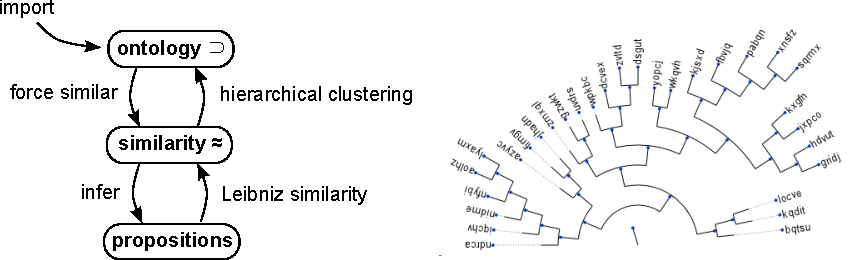
\includegraphics[scale=0.8]{ontology-relations-relations.pdf}
\caption{Left: relations between ontological data.  Right: a random example of dendrogram.}
\label{fig:ontology-relations-relations}
\end{figure}

\section*{Appendix: XXXX}
\end{comment}

\section*{致谢}

首先必须感谢 王培 \cite{Wang2006} \cite{Wang2013} 与 Ben Goertzel \cite{Goertzel2011} 对\textbf{通用人工智能} (AGI) 的重大贡献。  此外,我和 Abram Demski、Russell Wallace 花了很多年讨论各种关於逻辑的想法。  还有 Matt Mahoney 和其他在 AGI 电邮论坛上的参与者。 William Taysom、Seh、Joseph Cheung 帮手编写 Genifer 程式,现开源在 Github 上。

\bibliographystyle{plain} % or number or aaai ...
\bibliography{AGI-book}

\onecolumn

% Bigger figures

\end{document}
